  \section[FileMan Query Language (FMQL)]{FMQL}
  \label{sec:fmql}

  \initial{F}\textit{ileMan Query Language (FMQL)}\
  is a Query Language that provides access to both FileMan data\
  - a vital measurement of a patient - and the schema of that data - the type ``Vital Measurement''.\\
  
  \begin{figure}[ht!]
    \centering
    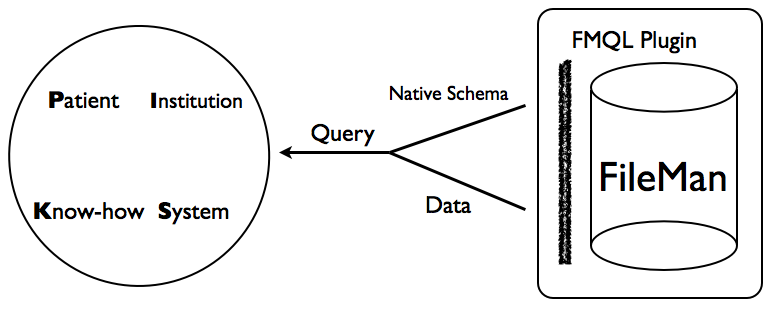
\includegraphics[scale=0.4]{fmqlFromFileMan.png}
    \caption{Querying data from Fileman~\cite[Fig.~1]{_fmql_framework_2013}}
    \label{fig:fmql}
  \end{figure}  

  \noindent The three things that it addresses are:
  \begin{enumerate}
    \item Identity: every entity and entity type in FileMan gets a unique identifier - a URI.
    \item Data Formats: a consistent form of JSON, the web-friendly response format, for every\
    type of data in the system as well as HTML for human readers and RDF for web-data practitioners.\
    \item Query Nuance: from the precise - SELECT - to the broader - DESCRIBE - or just COUNT, covers data hierarchies\
    and graphical layouts, paging and filtering.  \citep{_fmql_framework_2013}     
  \end{enumerate}
